\section{Distribution}

Like for its previous games, id decided to distribute Doom following the shareware model. A small part of the game would be given away for free and players were encouraged to be copied and redistributed as much as possible. If they liked the game they could send monet directly to id Software and receive the full version.\\
\par
\cfullimage{endoom.png}{Leaving the game displays instructions to buy the game.}
\par
Ideally, to make distribution as easy as possible, the game would have fitted on one 3\nicefrac{1}{2}-inch floppy disk. Even though 650 KiB floppy reader were fading out in favor of 1,440 KiB floppies, because of the volume of assets, DooM shareware still used two disks.\\
\cfullimage{floppies.png}{Two floppies containing Doom shareware.}
\par
In the previous photo, notice how the shareware came with a guide book which had little to do with id Software. In order to maximize distribution, id Software encouraged retails and distributor to sell the shareware or embedd it however they wanted.\\
\par

\fq{The challenge was: "How do we get Doom in the store? How do we get something free on shelves?\\
par 
The idea was that the title screen of doom says "Suggested retail price \$9 dollars" on it and then we told the
companies that were already in the stores "if you put DOOM in the store in a box on the shelf you just keep all
the money. We don't want any of it just put it in a box and sell it".\\
\par 
Nutty, except that worked. It was everywhere. If you went into a CompUSA back then in 1994 you would see ten different boxes of doom and think they're all different games but they're all the same shareware game. Distributors ended up trying to make the best looking boxes to outperform their competitors because all they were allowed to sell was the shareware.}{John Romero}

\subsection{What's in the disk?}

\par
INCLUDE A DOS DIS OF A FRESH INSTALL OF DOOM.
\par

\def\angle{0}
\def\radius{3}
\def\cyclelist{{"orange","blue","red","green"}}
\newcount\cyclecount \cyclecount=-1
\newcount\ind \ind=-1
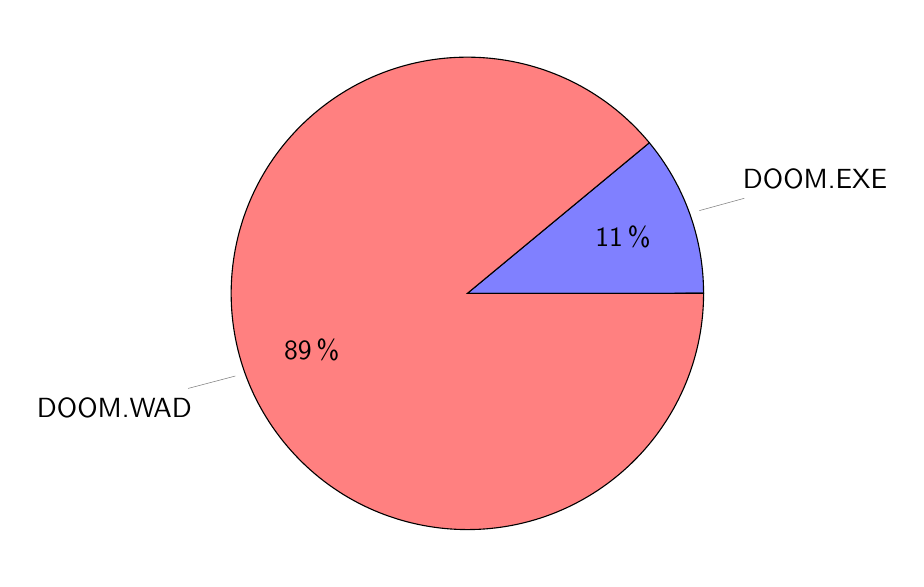
\begin{tikzpicture}[nodes = {font=\sffamily}]
  \foreach \percent/\name in {
      11/DOOM.EXE,
      89/DOOM.WAD
    } {
      \ifx\percent\empty\else               % If \percent is empty, do nothing
        \global\advance\cyclecount by 1     % Advance cyclecount
        \global\advance\ind by 1            % Advance list index
        \ifnum3<\cyclecount                 % If cyclecount is larger than list
          \global\cyclecount=0              %   reset cyclecount and
          \global\ind=0                     %   reset list index
        \fi
        \pgfmathparse{\cyclelist[\the\ind]} % Get color from cycle list
        \edef\color{\pgfmathresult}         %   and store as \color
        % Draw angle and set labels
        \draw[fill={\color!50},draw={black}] (0,0) -- (\angle:\radius)
          arc (\angle:\angle+\percent*3.6:\radius) -- cycle;
        \node at (\angle+0.5*\percent*3.6:0.7*\radius) {\percent\,\%};
        \node[pin=\angle+0.5*\percent*3.6:\name]
          at (\angle+0.5*\percent*3.6:\radius) {};
        \pgfmathparse{\angle+\percent*3.6}  % Advance angle
        \xdef\angle{\pgfmathresult}         %   and store in \angle
      \fi
    };
\end{tikzpicture}
\par
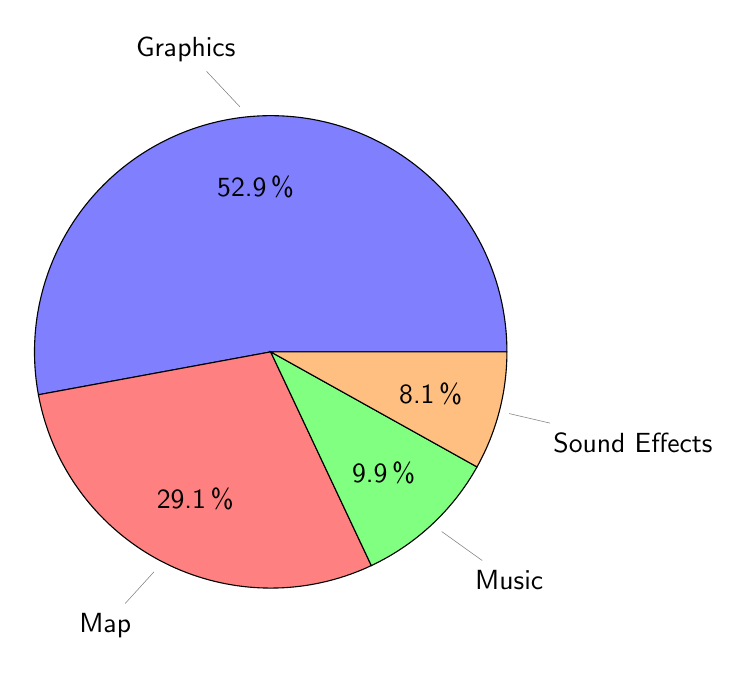
\begin{tikzpicture}[nodes = {font=\sffamily}]
  \foreach \percent/\name in {
      52.9/Graphics,
      29.1/Map,
       9.9/Music,
       8.1/{Sound Effects},
    } {
      \ifx\percent\empty\else               % If \percent is empty, do nothing
        \global\advance\cyclecount by 1     % Advance cyclecount
        \global\advance\ind by 1            % Advance list index
        \ifnum3<\cyclecount                 % If cyclecount is larger than list
          \global\cyclecount=0              %   reset cyclecount and
          \global\ind=0                     %   reset list index
        \fi
        \pgfmathparse{\cyclelist[\the\ind]} % Get color from cycle list
        \edef\color{\pgfmathresult}         %   and store as \color
        % Draw angle and set labels
        \draw[fill={\color!50},draw={black}] (0,0) -- (\angle:\radius)
          arc (\angle:\angle+\percent*3.6:\radius) -- cycle;
        \node at (\angle+0.5*\percent*3.6:0.7*\radius) {\percent\,\%};
        \node[pin=\angle+0.5*\percent*3.6:\name]
          at (\angle+0.5*\percent*3.6:\radius) {};
        \pgfmathparse{\angle+\percent*3.6}  % Advance angle
        \xdef\angle{\pgfmathresult}         %   and store in \angle
      \fi
    };
\end{tikzpicture}